\section{Real Time Trajectory Prediction Using Deep Conditional
Generative Models}\label{header-n953}

\emph{IEEE ROBOTICS AND AUTOMATION LETTERS, VOL. 5, NO. 2, APRIL 2020}
{[}36{]}

\subsection{Introduction}\label{header-n955}

Dynamic high-speed robotics tasks often require accurate methods to
forecast the future value of a physical quantity and these methods must
respect the application's real-time constraints. For example, to hit or
catch a flying ball, a robot needs to predict accurately and fast the
trajectory of the ball. Note that the time it takes to compute the
predictions, called \emph{latency}, is as important for the application
as the accuracy in the prediction. Physics-based models are often used
to trajectory forecasting because of their velocity in making a
prediction. Despite this, in some applications, the best known
physics-based model is not accurate enough or, even if the physics is
accurate, estimating all its relevant variables can be difficult. On the
other hand, a data-driven model could overcome these limitations and,
generally, their predictions are more accurate. However, the modern
data-driven approaches, like those based on recurrent neural networks,
suffer from cumulative errors. This work proposes a novel method for
trajectory prediction that mixes the power of deep learning and
conditional generative models to provide a data-driven approach for
accurate trajectory forecasting with the low latency required by
real-time applications. The system is tested using a table tennis
system, in which two robotic arms has to correctly hit a ball. The
figure below shows this system.

\begin{figure}[h!]
\centering
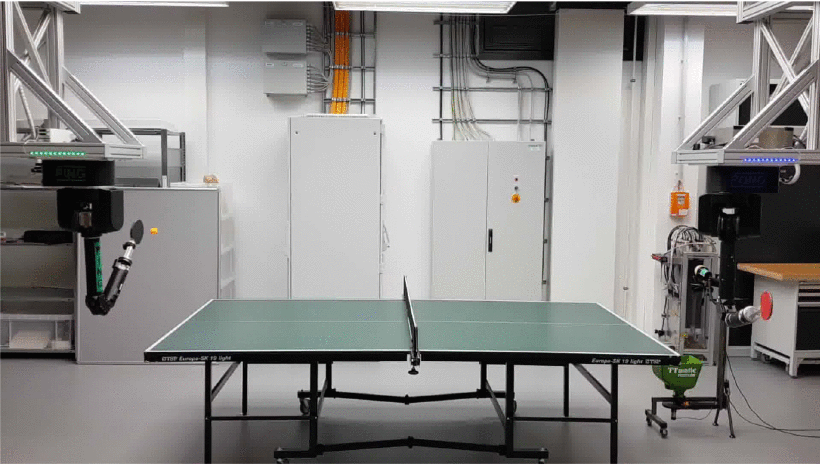
\includegraphics[width=0.7\linewidth]{images/tabletennis.png}
\caption{Table tennis robotic system}
\end{figure}

\subsection{Proposed method}\label{header-n958}

\subsubsection{Trajectory definition}\label{header-n959}

The term trajectory is commonly used to refer to a realization of a time
series or Markov decision process. A trajectory is defined as
$\tau=\{y_t^{n}\}^{T_n}_{t=1}$, where $T_n$ is a sequence of
multiple observations $y_t^{n}$ ($n$ represents the time and $t$
is the index of a trajectory in the data set). For the tennis example,
an observation $y^{n}_t$ is a three-dimensional vector representing
the ball position at time $t$ of the ball trajectory $n$. Each
trajectory $\tau_n∼ P(\tau)$ is assumed to be independently sampled
from the trajectory distribution $P(\tau)$. Formally, the goal of
trajectory forecasting is to compute the conditional distribution
$p(y_t,..., y_T | y_1,..., y_{t−1})$, representing the distribution of
the future values of a trajectory $\{y_t,..., y_T \}$ given the
previous observations $\{y_1,...., y_{t-1}\}$ ($y_t$ is a random
variable representing the observation indexed by time $t$ in any
trajectory). Some models use the factorization property of probability
theory
\newline
$ p(\boldsymbol{y}_{t:T} \, | \,\boldsymbol{y}_{1:t-1}) = \prod _{i=t}^{T}{p(\boldsymbol{y}_{i} \, | \,\boldsymbol{y}_{1:i-1})}, $
\newline
but they predict directly a single observation, while the others are
calculated by using the past predictions as input. This is a
\emph{recursive} approach: it uses its predictions as input to predict
farther into the future. These approaches can predict sequences of
arbitrary length, but they have the disadvantage that errors are
cumulative. However, for trajectory prediction in physical systems,
where we are measuring all the relevant variables, the authors would
expect long term prediction to be more accurate. In fact, this is not
true and even a data-driven model, implemented for example with LTSM, is
heavily penalized by the cumulative error, that renders long term
predictions less accurate.

\subsubsection{Deep conditional generative models}\label{header-n963}

The goal is to find a way to represent the conditional distribution
$p(y_{t:T} | y_{1:t−1})$ directly, in a way where the model
predictions are not fed back into the model. In addition, we want to use
a powerful model that can capture non-linear relationships between the
future and past observations. To do this, a complex non-linear
regression model, such as a neural network, can be used. The authors use
two auxiliary input variables $x^{t}$ and $\hat x^{t}$ that
represent a zero-padded input observation and an observation mask. In
particular, $x^{t} = 1$ represent the observations viewed so far,
while the non-observed parts of the trajectory are tagged with
$x^{t} = 0$. Similarly, the variable $\hat x^{t} \in \{0, 1\}$
indicates which values were observed and which values were not. Using
the auxiliary variables the model can make predictions with any number
of input observations $t \in \{0, 1,...,T\} $. The proposed approach
assumes a fixed maximum prediction horizon $T$ for all trajectories.

\subsubsection{Capturing Uncertainty and Variability}\label{header-n965}

Quantifying the uncertainty of the trajectory predicted by the model is
important for decision making. In robot table tennis, for example, the
robot could wait for more ball observations if there is high uncertainty
about the ball trajectory, but waiting too long will result in failure
to hit the ball. Uncertainty can be captured using a latent variable
$z_n$, that can be mapped to a trajectory using a complex non-linear
function. The authors want to emphasize that the limitation of a fixed
prediction horizon $T$ means that prediction beyond $T$ can't be
done, but the model can be trained with trajectories of any length
$T_n$. The proposed approach is based on variational auto-encoders.
The decoder network takes as input the previous observations
$y_{1:t−1}$ represented by $(x^{t} , \hat x^{t} )$ as well as the
latent variable $z$ that encodes one of the possible future
trajectories $\hat y$ (which contains the predicted future
observations $y_{t:T}$. The encoder network produces the variational
distribution $q\varphi(z | y1:t)$, which is a partial trajectory with
observations $y_{1:t}$ to the latent space $z$.

\begin{figure}[h!]
\centering
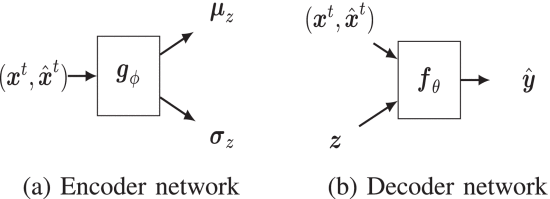
\includegraphics[width=0.8\linewidth]{images/encdec.png}
\caption{Encoder and decoder networks for the proposed approach}
\end{figure}

\subsubsection{Inference and training procedure}\label{header-n968}

At prediction time, the encoder computes the latent space distribution
using the given past observations. It produces a mean $\mu_z$ and a
standard deviation $\sigma_z$. Next, several values
$z^l \sim {\mathcal N}(z | \mu_z, \sigma_z)$ are sampled and they are
passed, with the past observations, to the decoder module to predict the
future trajectory. The training set consists of a set of trajectories
$\tau_n$ each of a possibly different length $T_n$. Sampled
mini-batches are used to train the model: for any trajectory, a cut
point $t : 0 <t $ is randomly selected and the lower bound for
$p(y_{t:T} | y_{1:t−1})$ is computed for the particular $t$. In this
way, the model will learn to make predictions for any number of given
observations, including an empty set. Finally, to make our model more
robust, the authors randomly generate missing observations and outliers
for the previous observations $y_{1:t−1}$ in each of the trajectories
included in the training mini-batch. To generate outliers, an
observation is simply replaced with a random value within the input
domain.

\subsection{Experiments}\label{header-n970}

The authors evaluate the proposed method (which predicts the trajectory
of a table tennis ball) both in a real and simulated system. The
proposed method is called "TVAE" (Trajectory Variational Auto-Encoder).
The metric measured is the prediction error and latency. The baseline
methods, used to compare and evaluate the performance of the proposed
method, are an LTSM and the physics-based approach. The ball's physics
is described in {[}37{]}, while the initial velocity and position are
calculated as described in {[}38{]}. The latter method consists of
fitting a polynomial to the first $n$ observations and evaluating the
polynomial of degree $k$ and its derivative in $t = 0$. These
parameters are set to $n = 30$ and $k = 2$, that provided the
highest predictive performance on the training data set.

\subsubsection{Prediction accuracy in simulation}\label{header-n972}

The results should be optimal for the physics-based model on simulation,
where the only source of error is the initial position and velocity
estimation from noisy ball observations. The authors generated 2000 ball
trajectories for training and another 200 for the test. The training
results obtained in a simulated environment are plotted in the following
figure. In simulation, the error distribution of the proposed method and
the physics-based model is almost identical. The results of the LSTM are
slightly better than the proposed model for the first 10 observations,
but the error for long term prediction grows uncontrollably.

\begin{figure}[h!]
\centering
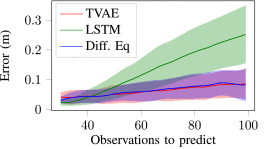
\includegraphics[width=0.37\linewidth]{images/accuracyballres.png}
\caption{Distribution of the error in the test set for simulated data as a function of the number of observations}
\end{figure}

\subsubsection{Prediction accuracy in the real
system}\label{header-n975}

There are several issues that make ball prediction harder on the real
system: there are missing observations, the error is not the same in all
the space due to the effects of lens distortion, and the ball spin can
not be observed directly. The training set has 614 samples, while the
test set is composed of 35 trajectories. All samples are collected in a
real environment: the ball is thrown using the hand, using a mechanical
launcher, and hitting them with a table tennis racket. Since the
trajectories have typically a duration between 0.8 and 1.2 seconds, the
time horizon is set to $T = 1.2$ seconds. The figure below shows the
training results obtained using real-time data. The proposed method
outperforms the long term prediction accuracy of the other models. The
LSTM, as expected, is very precise at the beginning but starts to
accumulate errors and becomes quickly less accurate. The physics-based
model is in the middle: more accurate than the LTSM approach but less
accurate than TVAE.

\begin{figure}[h!]
\centering
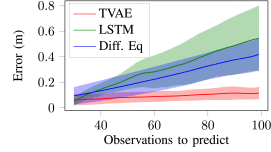
\includegraphics[width=0.37\linewidth]{images/accuracyballresreal.png}
\caption{Distribution of the error in the test set for real data as a function of the number of observations}
\end{figure}

\subsubsection{A real robot table tennis system}\label{header-n978}

The authors implemented the proposed method in a real robot table tennis
system, to test the performance in a real game. To do this, they
modified the ProMP approach {[}39{]} to use the proposed ball model.
ProMP works as follows:

\begin{itemize}
\item
  first, the initial time and duration of the movement primitive are
  computed by maximizing the likelihood of hitting the ball;
\item
  second, the movement primitive is adapted to hit the ball using a
  probability distribution by conditioning the racket distribution to
  intersect the ball distribution;
\item
  third, to avoid dangerous movements, the robot does not hit if the
  likelihood is lower than a certain threshold.
\end{itemize}

To compute the ball distribution, the authors took 30 trajectory samples
from the proposed model and computed empirically its mean and
covariance. The adapted method obtained a hitting rate of 98.9\%
compared to 96.7\% obtained using a ProMP. This experiment also shows
that the presented approach can be used in a system with hard real-time
constraints. The proposed system can infer the future ball trajectory
from past observations with a latency between 8 ms and 10 ms.